\documentclass{article}
\usepackage{geometry}
 \geometry{
 a4paper,
 total={170mm,257mm},
 left=20mm,
 top=20mm,
 }
\usepackage[english,greek, main=greek]{babel}
\usepackage[utf8]{inputenc}
\usepackage{amsmath}
\usepackage{graphicx} % for graphics and plots
\usepackage{subcaption} % for subfigures and subcaptions and \ContinuedFloat
\usepackage{placeins} % for \FloatBarrier
\usepackage{xcolor} % for colour definitions
\usepackage{listings} % for code highlighting
\usepackage{verbatim} % for file input
\usepackage{hyperref} % clickable links
\usepackage{datatool} % for csv reading

\newcommand{\eng}[1]{\foreignlanguage{english}{#1}} % shortcut for inserting english into greek text

\useshorthands{;}
\defineshorthand{;}{?} % greek question mark instead of english semicolon


\title{
    \includegraphics[width=\textwidth]{~/Pictures/emp.png} \\
    \vskip 5cm
    Κατανεμημένα Συστήματα \\
    \large Εξαμηνιαία Εργασία - \eng{BlockChat} 
    \vskip 5cm
}

\author{ Αναστάσιος Στέφανος Αναγνώστου \\ \large 03119051 }

\begin{document}

\maketitle \clearpage \tableofcontents \clearpage

\part{Σχεδιασμός Συστήματος}

\section{Δεν είμαι σίγουρος}

\clearpage
\part{Πειράματα}

\section{Απόδοση του συστήματος}

Ανά πείραμα αξιολογούνται, αφενός τα πιο χρονοβόρα κομμάτια του κώδικα, όπως
υποδεικνύει το \eng{profiling} καθενός κόμβου κατά την εκτέλεση του πειράματος,
αφετέρου οι συναρτήσεις \eng{mint}, \eng{validateTransaction} και
\eng{processTXs}, οι οποίες συνιστούν την λογική λειτουργίας των κόμβων του
συστήματος.

Σημειώνεται ότι το ποσοστό του χρόνου εκτέλεσης των σημείων που υποδεικνύει το
\eng{profiling} δεν είναι κληρονομημένο, δηλαδή δεν εμπεριέχονται στο ποσοστό
οι χρόνοι εκτέλεσης των συναρτήσεων που καλούνται από τις συναρτήσεις που
εμφανίζονται στο \eng{profiling}.

\subsection{Ρυθμαπόδοση}

Στο πείραμα για την αξιολόγηση της ρυθμαπόδοσης του συστήματος, στήνεται ένα
δίκτυο 5 κόμβων, καθένας εκ των οποίων εκτελεί 1 \eng{staking} συναλλαγή και 50
συναλλαγές (συγκεκριμένα αποστολές μηνυμάτων) προς τους άλλους κόμβους. Η
ταχύτητα αποστολής συναλλαγών είναι ίδια μεταξύ των κόμβων, ίση με
$10\frac{txs}{s}$ και παραμένει σταθερή μεταξύ όλων των πειραμάτων.

Το πρώτο πράγμα που φαίνεται στο σχήμα \ref{fig:throughput-cost-centers} είναι
ότι το μακράν πιο χρονοβόρο μέρος του κώδικα είναι η συνάρτηση
\eng{modular\_exponentiation} που χρησιμοποιείται γενικά για την κρυπτογράφηση
/ αποκρυπτογράφηση και υπογραφή / επαλήθευση μηνυμάτων. Συγκεκριμένα, φαίνεται
να λαμβάνει περίπου το 50\% του συνολικού χρόνου εκτέλεσης του προγράμματος.

\graphicspath{{../experiments/profiled\_outputs/throughputdel100ms/}}

\begin{figure}[ht]
    \centering
    \begin{subfigure}{\textwidth}
        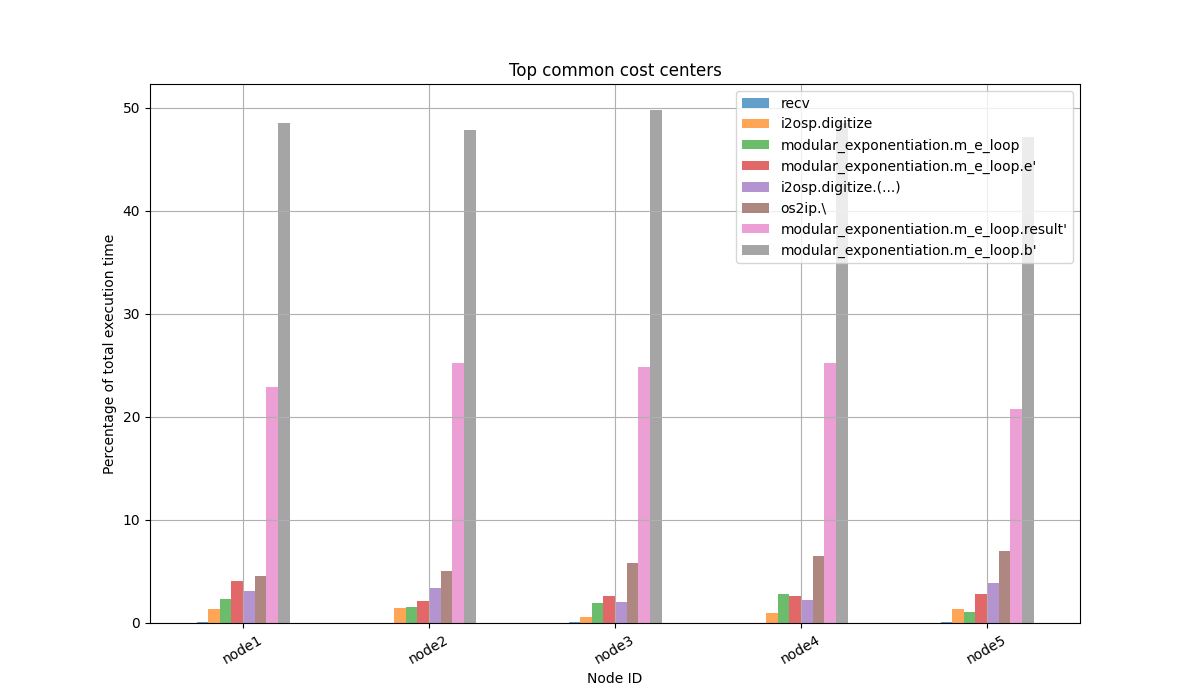
\includegraphics[width=\textwidth]{./capacity5/cost-centers-capacity5.png}
        \caption{\eng{capacity=5}}
    \end{subfigure}
\end{figure}
\begin{figure}[ht]
    \ContinuedFloat
    \begin{subfigure}{\textwidth}
        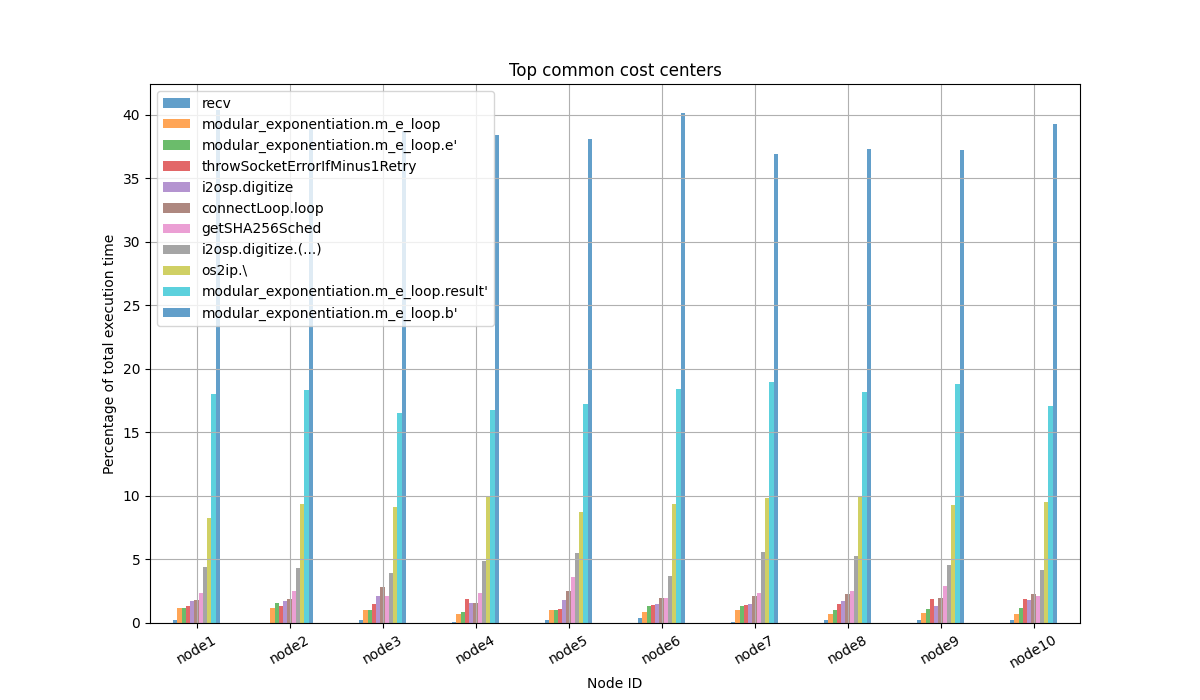
\includegraphics[width=\textwidth]{./capacity10/cost-centers-capacity10.png}
        \caption{\eng{capacity=10}}
    \end{subfigure}
    \begin{subfigure}{\textwidth}
        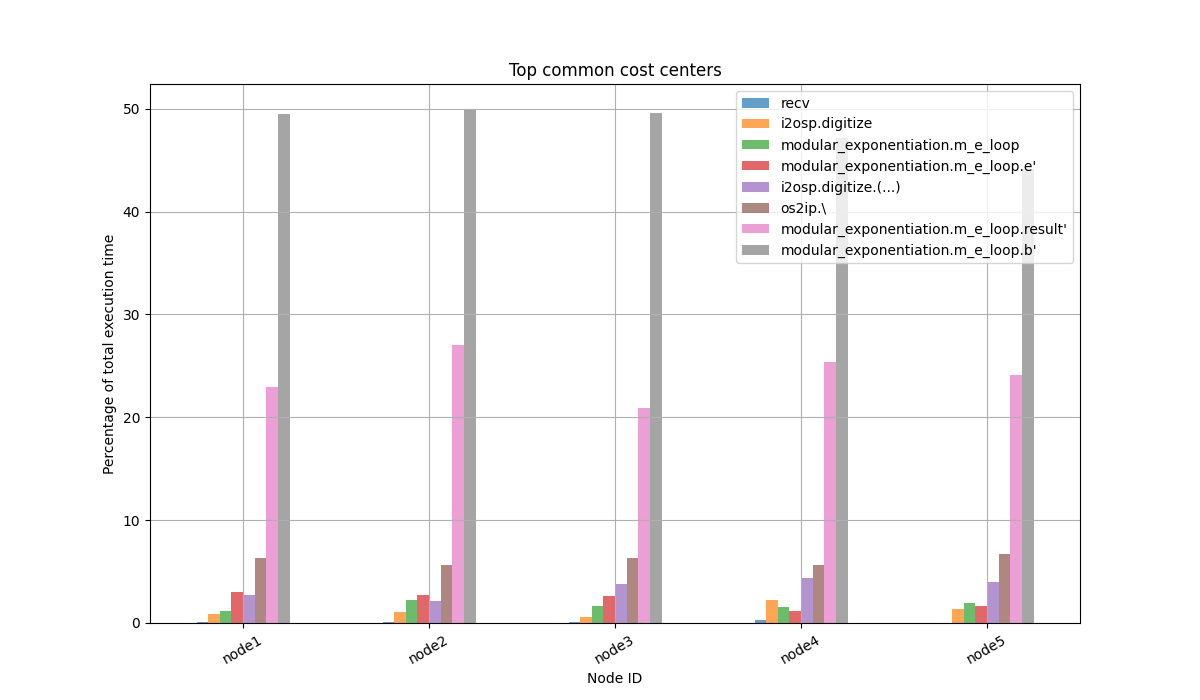
\includegraphics[width=\textwidth]{./capacity20/cost-centers-capacity20.png}
        \caption{\eng{capacity=20}}
    \end{subfigure}
    \caption{Τα πιο χρονοβόρα κομμάτια του κώδικα}
    \label{fig:throughput-cost-centers}
\end{figure}
\FloatBarrier

Στον πίνακα \ref{tab:throughput-funcs} παρουσιάζονται ορισμένα στατιστικά σχετικά
με τις συναρτήσεις \eng{mint}, \eng{validateTransaction} και \eng{processTXs}.
Το πιο σημαντικό να παρατηρηθεί είναι ότι, για κάθε κόμβο, οι κλήσεις στην συνάρτηση
\eng{validateTransaction} είναι ακριβώς τόσες όσες και οι συναλλαγές που αποστέλλονται
από όλους τους κόμβους $\left(5 + 5 \times 50 = 255 \right)$. Επίσης, $\#mint +
\#validateTransaction = \#processTXs$ (η -1 διαφορά είναι επειδή έγινε η τελευταία κλήση
και τα προγράμματα έλαβαν σήμα τερματισμού). Αυτό σημαίνει ότι οι κόμβοι επιβεβαίωσαν
όλες τις συναλλαγές κατά την διάρκεια του πειράματος.

Εξαίρεση αποτελεί ο πίνακας \ref{tab:throughput-funcs-1}, όπου οι κόμβοι δεν προλαβαίνουν
να επιβεβαιώσουν όλες τις συναλλαγές που λαμβάνουν, αλλά εκκρεμούν 5 από τις 255. Αυτό
οφείλεται στην μικρή χωρητικότητα του \eng{block}, το οποίο σημαίνει ότι οι κόμβοι πρέπει
συχνά να καλούν την χρονοβόρα συνάρτηση \eng{mint} και να διακόπτουν την διαδικασία
επιβεβαίωσης.

Γενικά, παρατηρείται ότι, με κάποιες μικρές διακυμάνσεις, η \eng{processTXs}
καταναλώνει 9-10\% του συνολικού χρόνου εκτέλεσης, η \eng{mint} 1-3\% και
η \eng{validateTransaction} 5-7\%.

\begin{figure}[ht]
    \centering
    \begin{subfigure}{\textwidth}
        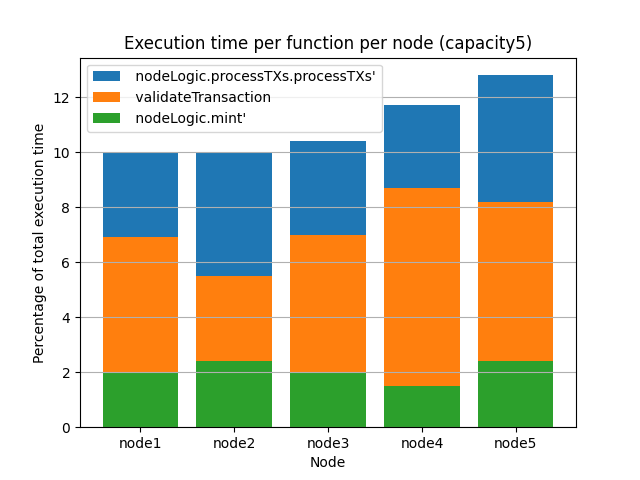
\includegraphics[width=\textwidth]{./capacity5/times_of_function_per_node_capacity5.png}
        \caption{Ρυθμαπόδοση \eng{capacity=5}}
    \end{subfigure}
\end{figure}
\begin{figure}[ht]
    \ContinuedFloat
    \begin{subfigure}{\textwidth}
        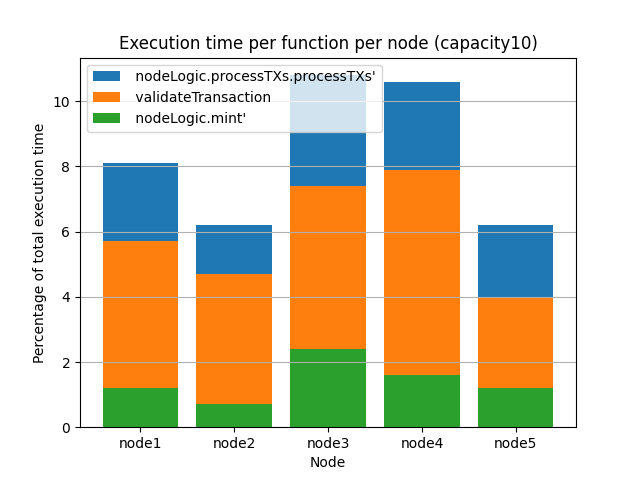
\includegraphics[width=\textwidth]{./capacity10/times_of_function_per_node_capacity10.png}
        \caption{Ρυθμαπόδοση \eng{capacity=10}}
    \end{subfigure}
    \begin{subfigure}{\textwidth}
        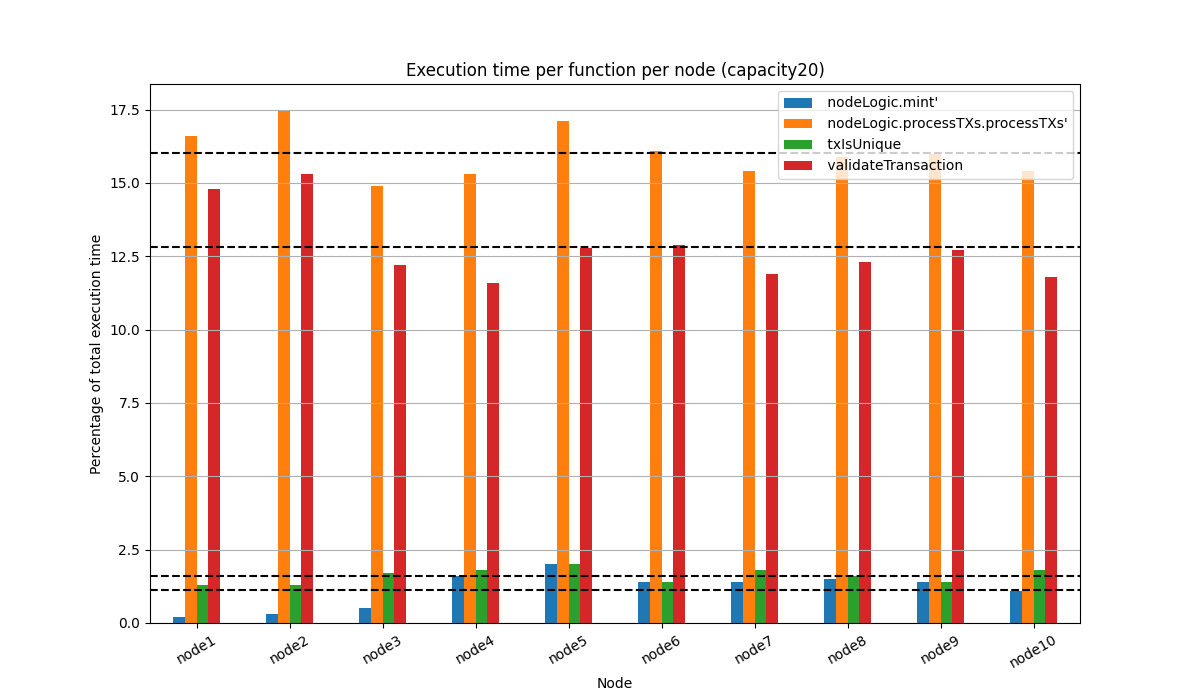
\includegraphics[width=\textwidth]{./capacity20/times_of_function_per_node_capacity20.png}
        \caption{Ρυθμαπόδοση \eng{capacity=20}}
    \end{subfigure}
    \caption{Ποσοστό χρόνου επί του συνολικού χρόνου εκτέλεσης που λαμβάνει η κάθε συνάρτηση}
\end{figure}
\FloatBarrier

\DTLloaddb{th-calls1}{../experiments/profiled_outputs/throughputdel100ms/capacity5/calls-latex.csv}
\DTLloaddb{th-calls2}{../experiments/profiled_outputs/throughputdel100ms/capacity10/calls-latex.csv}
\DTLloaddb{th-calls3}{../experiments/profiled_outputs/throughputdel100ms/capacity20/calls-latex.csv}

\begin{table}[ht]
    \caption{Στατιστικά συναρτήσεων ανά κόμβο} 
    \label{tab:throughput-funcs}
    \begin{subtable}{\textwidth}
        \centering
        \caption{\eng{capacity=5}}
        \label{tab:throughput-funcs-1}
        \selectlanguage{english}
        \DTLdisplaydb{th-calls1}
        \selectlanguage{greek}
    \end{subtable}
\end{table}

\begin{table}[ht]
    \ContinuedFloat
    \begin{subtable}{0.45\textwidth}
        \centering
        \caption{\eng{capacity=10}}
        \label{tab:throughput-funcs-2}
        \selectlanguage{english}
        \DTLdisplaydb[MemInh]{th-calls2}
        \selectlanguage{greek}
    \end{subtable}
    \hfill
    \begin{subtable}{0.45\textwidth}
        \centering
        \caption{\eng{capacity=20}}
        \label{tab:throughput-funcs-3}
        \selectlanguage{english}
        \DTLdisplaydb[File,Function,MemInh]{th-calls3}
        \selectlanguage{greek}
    \end{subtable}
\end{table}
\FloatBarrier

Στον πίνακα \ref{tab:throughput-funcs} φαίνεται ότι, με εξαίρεση λίγους κόμβους
στο πείραμα χωρητικότητας 5, το δίκτυο φτάνει εντός πειράματος σε σταθερή κατάσταση,
έχοντας επαληθεύει όλες τις συναλλαγές. Αυτό σημαίνει ότι η ρυθμαπόδοση του
συστήματος μπορεί να υπολογιστεί για κάθε πείραμα ως εξής:

\begin{equation}
    \text{Ρυθμαπόδοση} = \frac{\text{Συνολικές συναλλαγές}}{\text{Συνολικός χρόνος}} \Rightarrow \\
    \boxed{
        \begin{gathered}
            th_{capacity=5} = \frac{255}{5} = 51\frac{txs}{s} \\
            th_{capacity=10} = \frac{510}{5} = 102\frac{txs}{s} \\
            th_{capacity=20} = \frac{1010}{5} = 202\frac{txs}{s}
        \end{gathered}
        }
\end{equation}

\subsection{\eng{Block Time}}

Ομοίως μπορεί να εκτιμηθεί και το μέσο \eng{block time} του συστήματος:

\begin{equation}
    \begin{gathered}
        \text{\eng{Block Time}} = \frac{\text{Συνολικός χρόνος}}{\text{Συνολικά \eng{blocks}}} \Rightarrow
        \left\{
            \begin{gathered}
                bt_{capacity=5} = \frac{0.4 \times 46 + 0.6 \times 45}{5} \\ 
                bt_{capacity=10} = \frac{0.8 \times 22 + 0.2 \times 23}{5} \\ 
                bt_{capacity=20} = \frac{11}{5} \\
            \end{gathered} \right\}\Rightarrow \\ 
        \boxed{
            \begin{gathered}
                bt_{capacity=5} = 9.08\frac{blocks}{s} \\
                bt_{capacity=10} = 4.44\frac{blocks}{s} \\
                bt_{capacity=20} = 2.2\frac{blocks}{s}
            \end{gathered}
        }
    \end{gathered}
\end{equation}

\clearpage
\section{Κλιμακωσιμότητα του συστήματος}

Στα γραφήματα \ref{fig:scalability-cost-centers} φαίνονται τα πιο χρονοβόρα
κομμάτια του κώδικα για κάθε πείραμα κλιμακωσιμότητας. Φαίνεται ότι αυτά είναι
τα ίδια με τα πιο χρονοβόρα κομμάτια του κώδικα για το πείραμα ρυθμαπόδοσης,
με την συνάρτηση \eng{modular\_exponentiation} περίπου το 50\% του συνολικού
χρόνου εκτέλεσης του προγράμματος, αντί για το 40\% που ήταν προηγουμένως.

\graphicspath{{../experiments/profiled\_outputs/scalabilitydel100ms/}}

\begin{figure}[ht]
    \centering
    \begin{subfigure}{\textwidth}
        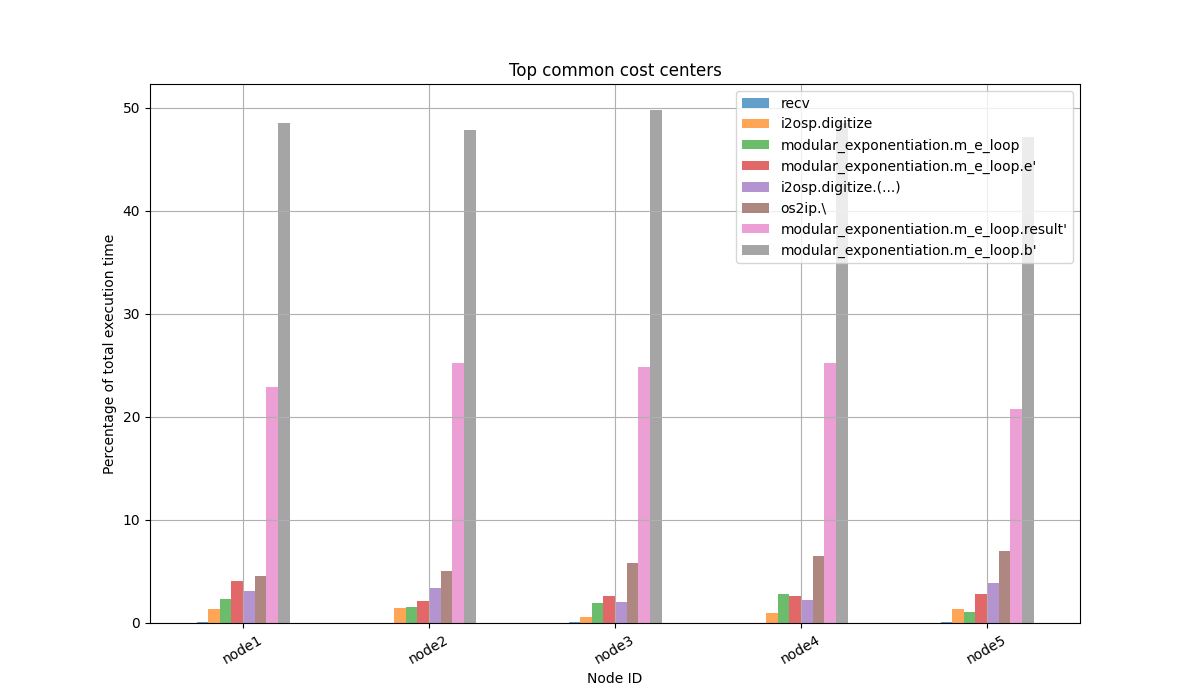
\includegraphics[width=\textwidth]{./capacity5/cost-centers-capacity5.png}
        \caption{\eng{capacity=5}}
    \end{subfigure}
\end{figure}
\begin{figure}[ht]
    \ContinuedFloat
    \begin{subfigure}{\textwidth}
        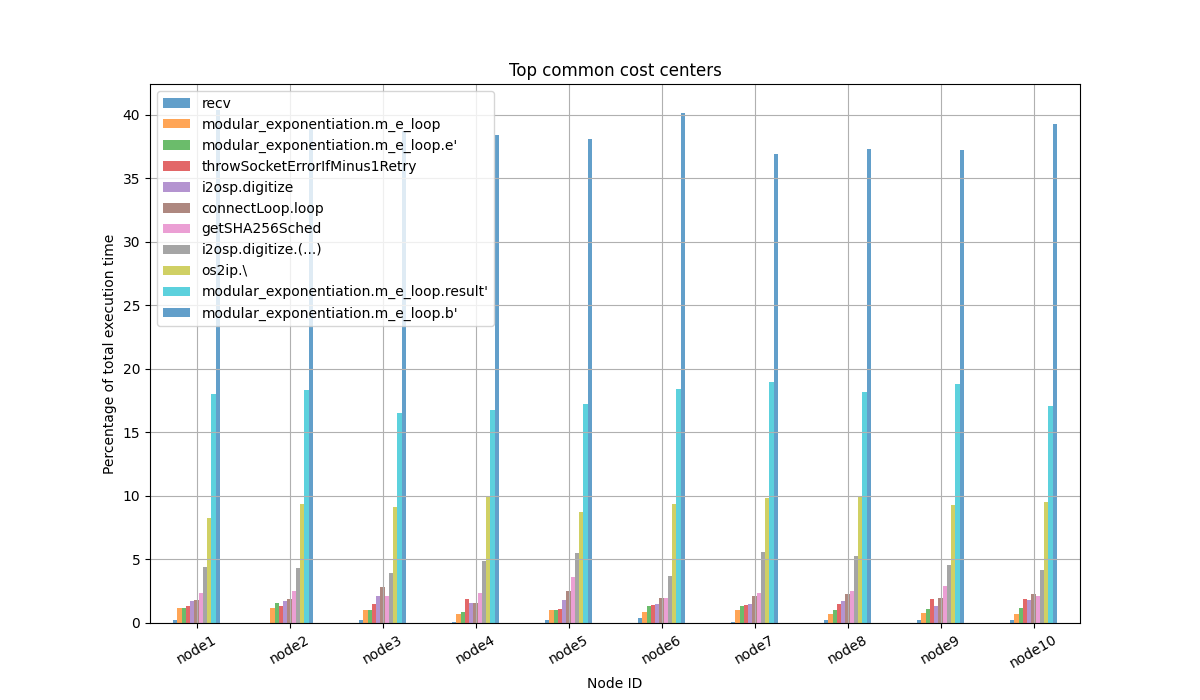
\includegraphics[width=\textwidth]{./capacity10/cost-centers-capacity10.png}
        \caption{\eng{capacity=10}}
    \end{subfigure}
    \begin{subfigure}{\textwidth}
        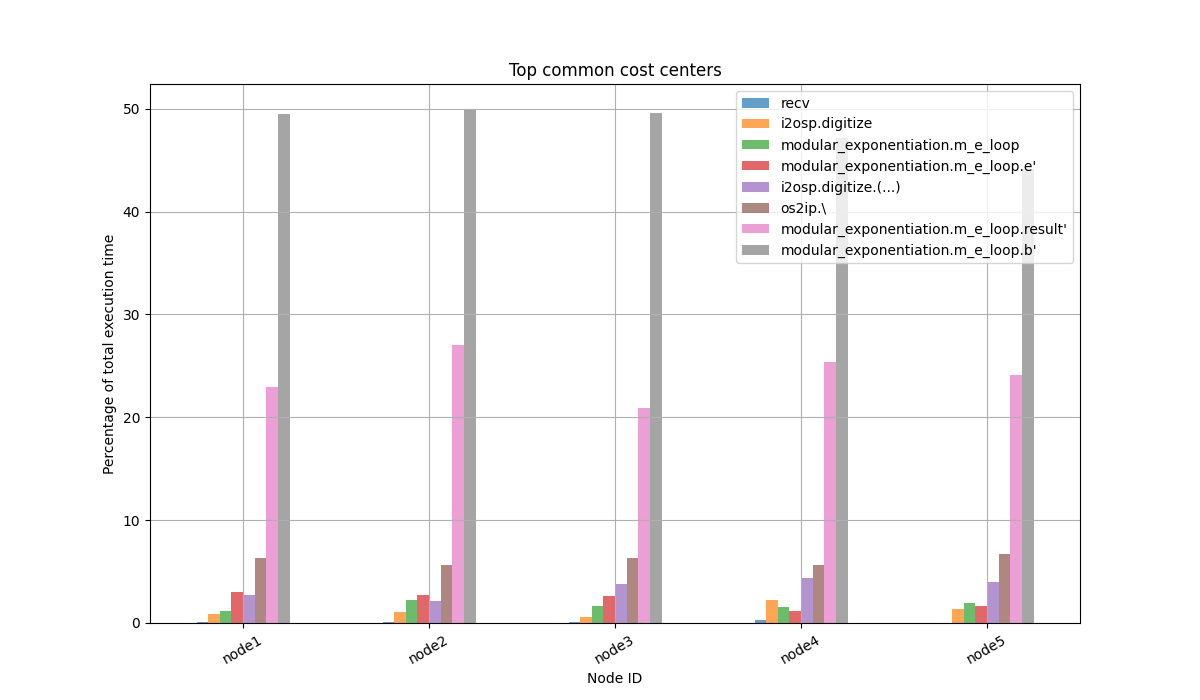
\includegraphics[width=\textwidth]{./capacity20/cost-centers-capacity20.png}
        \caption{\eng{capacity=20}}
    \end{subfigure}
    \caption{Τα πιο χρονοβόρα κομμάτια του κώδικα}
    \label{fig:scalability-cost-centers}
\end{figure}
\FloatBarrier

\DTLloaddb{sc-calls1}{../experiments/profiled_outputs/scalabilitydel100ms/capacity5/calls-latex.csv}
\DTLloaddb{sc-calls2}{../experiments/profiled_outputs/scalabilitydel100ms/capacity10/calls-latex.csv}
\DTLloaddb{sc-calls3}{../experiments/profiled_outputs/scalabilitydel100ms/capacity20/calls-latex.csv}

Στον πίνακα \ref{tab:scalability-funcs-1} φαίνονται οι κλήσεις ενδιαφέροντος
των κόμβων. Παρατηρώντας το πλήθος των κλήσεων ανά συνάρτηση, διαπιστώνεται ότι
οι κόμβοι δεν προλαβαίνουν να επικυρώσουν όλες τις συναλλαγές που λαμβάνουν.
Αυτό οφείλεται, αφενός στον μεγαλύτερο όγκο συναλλαγών $10 + 10 \times 100 =
1010$ το οποίο είναι $\approx 4$ φορές μεγαλύτερο από προηγουμένως, και
αφετέρου στην μικρή χωρητικότητα του \eng{block}, το οποίο σημαίνει ότι οι
κόμβοι πρέπει συχνά να καλούν την χρονοβόρα συνάρτηση \eng{mint} και να
διακόπτουν την διαδικασία επικύρωσης.

Επίσης, παρατηρείται ότι οι κόμβοι 7-8 έχουν μείνει πολύ πίσω σε σχέση
με τους υπόλοιπους κόμβους. Αυτό είναι μάλλον συνέπεια της πειραματικής
διάταξης, αφού όλοι οι κόμβοι τρέχουν στο ίδιο μηχάνημα.

\begin{table}[ht]
    \caption{Στατιστικά συναρτήσεων ανά κόμβο}
    \label{tab:scalability-funcs}
    \begin{subtable}{\textwidth}
        \centering
        \caption{\eng{capacity=5}}
        \label{tab:scalability-funcs-1}
        \selectlanguage{english}
        \DTLdisplaydb{sc-calls1}
        \selectlanguage{greek}
    \end{subtable}
\end{table}

Αντιθέτως, στους πίνακες \ref{tab:scalability-funcs-2} και \ref{tab:scalability-funcs-3}
φαίνεται από τις κλήσεις των συναρτήσεων ότι έχουν επικυρωθεί όλες οι συναλλαγές
και έχουν παραχθεί τα αντίστοιχα \eng{blocks}. Η μεγαλύτερη χωρητικότητα των
\eng{blocks} επιτρέπει στους κόμβους μεγαλύτερα χρονικά παράθυρα για την
επικύρωση των συναλλαγών και η διακοπή για την παραγωγή των \eng{blocks} δεν
καθυστερεί την εξέλιξη του δικτύου.

\begin{table}[ht]
    \ContinuedFloat
    \begin{subtable}{0.45\textwidth}
        \centering
        \caption{\eng{capacity=10}}
        \label{tab:scalability-funcs-2}
        \selectlanguage{english}
        \DTLdisplaydb[MemInh]{sc-calls2}
        \selectlanguage{greek}
    \end{subtable}
    \hfill
    \begin{subtable}{0.45\textwidth}
        \centering
        \caption{\eng{capacity=20}}
        \label{tab:scalability-funcs-3}
        \selectlanguage{english}
        \DTLdisplaydb[File,Function,MemInh]{sc-calls3}
        \selectlanguage{greek}
    \end{subtable}
\end{table}

Η ρυθμαπόδοση του συστήματος και το μέσο \eng{block time} μπορούν να υπολογιστούν όπως
προηγουμένως:

\begin{equation}
    \begin{gathered}
        \text{Ρυθμαπόδοση} = \frac{\text{Συνολικές συναλλαγές}}{\text{Συνολικός χρόνος}} \Rightarrow
        \left\{
            \begin{gathered}
                th_{capacity=5} = \frac{0.8 \times 62 + 0.2 \times 5}{10} \\
                th_{capacity=10} = \frac{1010}{10} \\
                th_{capacity=20} = \frac{1010}{10}
            \end{gathered}
        \right\} \Rightarrow \\
        \boxed{
            \begin{gathered}
                th_{capacity=5} = 5\frac{txs}{s} \\
                th_{capacity=10} = 101\frac{txs}{s} \\
                th_{capacity=20} = 101\frac{txs}{s}
            \end{gathered}
        }
    \end{gathered}
\end{equation}

\begin{equation}
    \begin{gathered}
        \text{\eng{Block Time}} = \frac{\text{Συνολικός χρόνος}}{\text{Συνολικά \eng{blocks}}} \Rightarrow
        \left\{
            \begin{gathered}
                bt_{capacity=5} = \frac{0.8 \times 12 + 0.2 \times 1}{10} \\ 
                bt_{capacity=10} = \frac{50}{10} \\ 
                bt_{capacity=20} = \frac{0.1 \times 22 + 0.1 \times 23 + 0.8 \times 25}{10} \\
            \end{gathered} \right\}\Rightarrow \\ 
        \boxed{
            \begin{gathered}
                bt_{capacity=5} = 0.962\frac{blocks}{s} \\
                bt_{capacity=10} = 5\frac{blocks}{s} \\
                bt_{capacity=20} = 2\frac{blocks}{s}
            \end{gathered}
        }
    \end{gathered}
\end{equation}

\begin{figure}[ht]
    \centering
    \begin{subfigure}{\textwidth}
        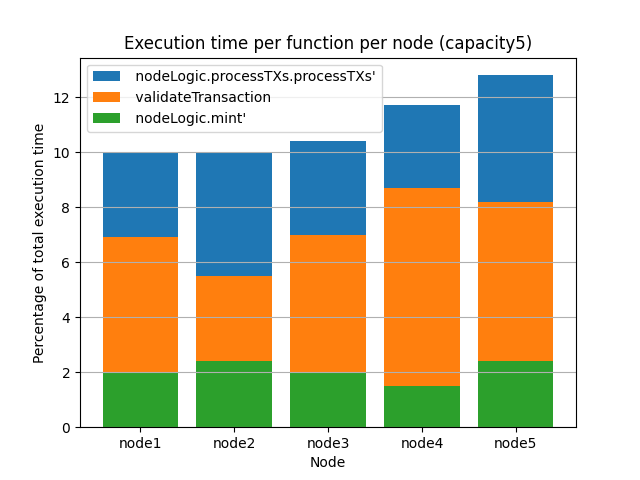
\includegraphics[width=\textwidth]{./capacity5/times_of_function_per_node_capacity5.png}
        \caption{\eng{capacity=5}}
    \end{subfigure}
\end{figure}
\begin{figure}[ht]
    \ContinuedFloat
    \begin{subfigure}{\textwidth}
        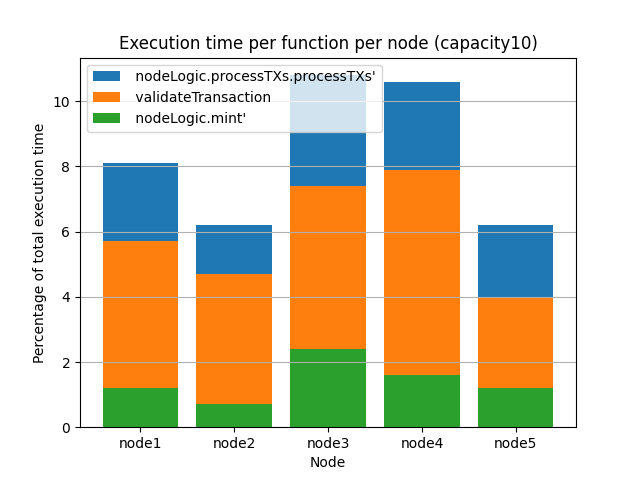
\includegraphics[width=\textwidth]{./capacity10/times_of_function_per_node_capacity10.png}
        \caption{\eng{capacity=10}}
    \end{subfigure}
    \centering
    \begin{subfigure}{\textwidth}
        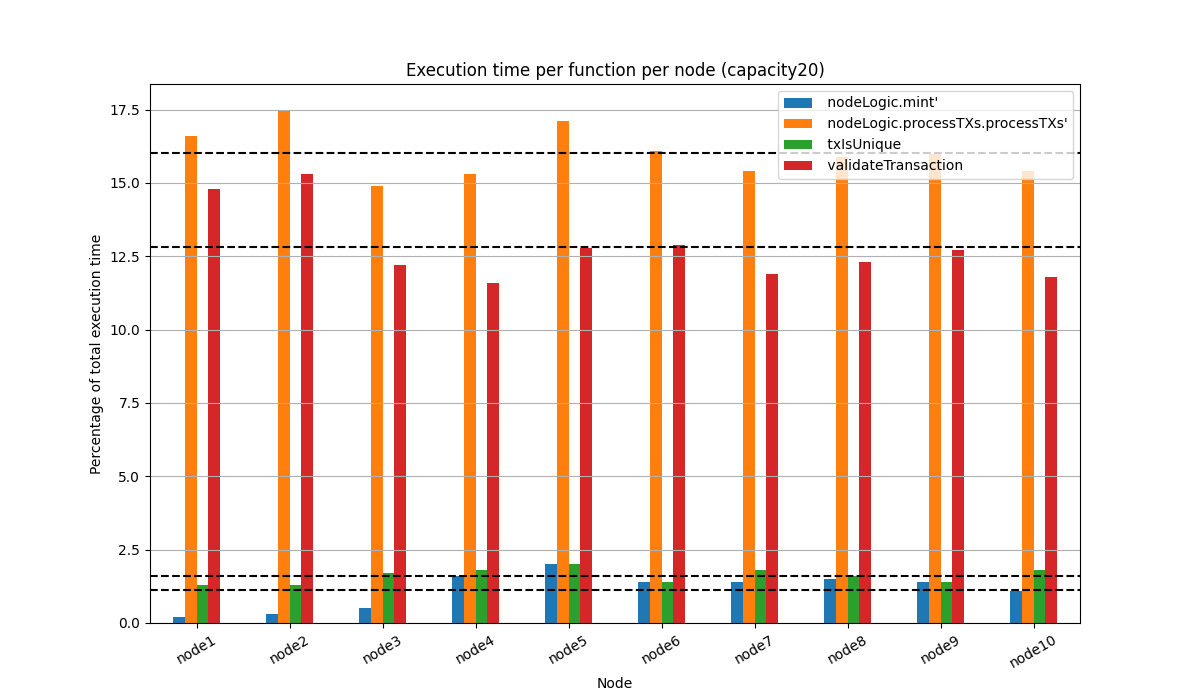
\includegraphics[width=\textwidth]{./capacity20/times_of_function_per_node_capacity20.png}
        \caption{\eng{capacity=20}}
    \end{subfigure}
    \caption{Ποσοστό χρόνου επί του συνολικού χρόνου εκτέλεσης που λαμβάνει η κάθε συνάρτηση}
\end{figure}
\FloatBarrier

\section{Δικαιοσύνη}

\graphicspath{{../experiments/profiled\_outputs/fairnessdel100ms/}}

\begin{figure}[ht]
    \centering
    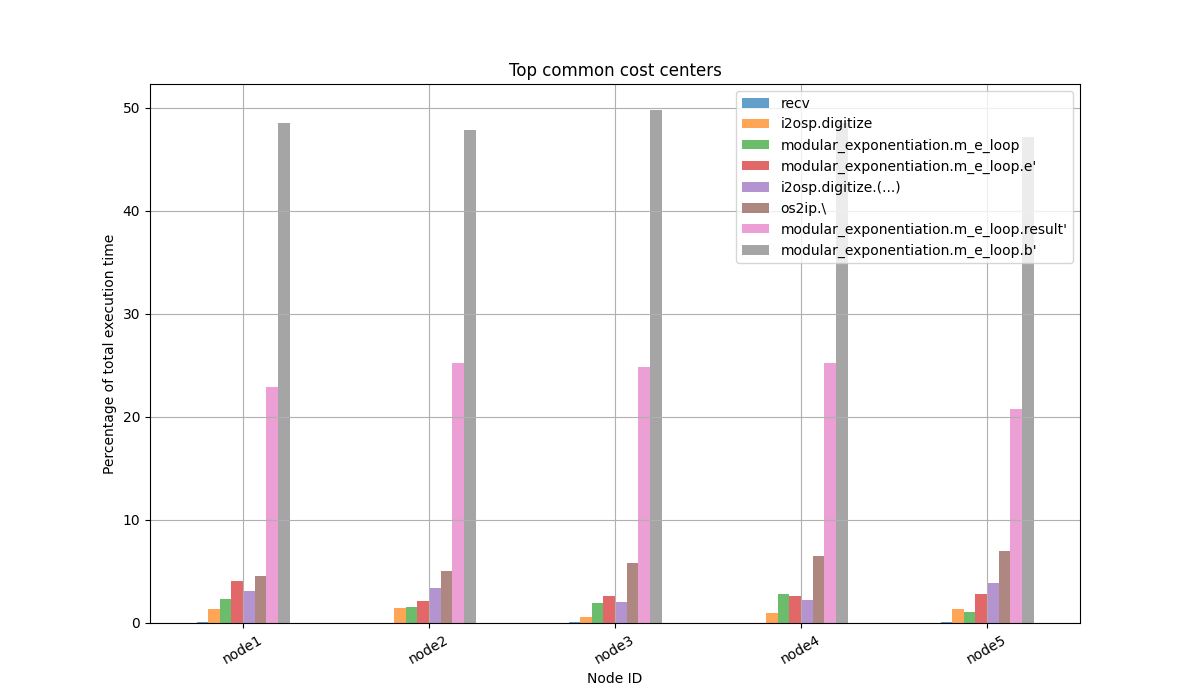
\includegraphics[width=\textwidth]{./capacity5/cost-centers-capacity5.png}
    \caption{Τα πιο χρονοβόρα κομμάτια του κώδικα \eng{capacity=5}}
    \label{fig:fairness-cost-centers}
\end{figure}

Στον πίνακα \ref{tab:fairness-funcs} φαίνονται οι κλήσεις μερικών συναρτήσεων
ενδιαφέροντος. Φαίνεται ότι τα πλήθη όλων των κλήσεων είναι ίδια ανά κόμβο,
πράγμα που σημαίνει ότι οι κόμβοι εκτελούν τις ίδιες λειτουργίες με την ίδια
συχνότητα. Παρ'όλα αυτά, ο κόμβος με το μεγαλύτερο \eng{stake} καταναλώνει πολύ
περισσότερο χρόνο στην συνάρτηση \eng{mint'} σε σχέση με τους υπόλοιπους
κόμβους, όπως φαίνεται και στο σχήμα \ref{fig:fairness-funcs}.

\DTLloaddb{fairness-calls}{../experiments/profiled_outputs/fairnessdel100ms/capacity5/calls-latex.csv}
\begin{table}[ht]
    \centering
    \caption{Στατιστικά συναρτήσεων ανά κόμβο \eng{capacity=5}}
    \label{tab:fairness-funcs}
    \selectlanguage{english}
    \DTLdisplaydb{fairness-calls}
    \selectlanguage{greek}
\end{table}

\begin{figure}[ht]
    \centering
    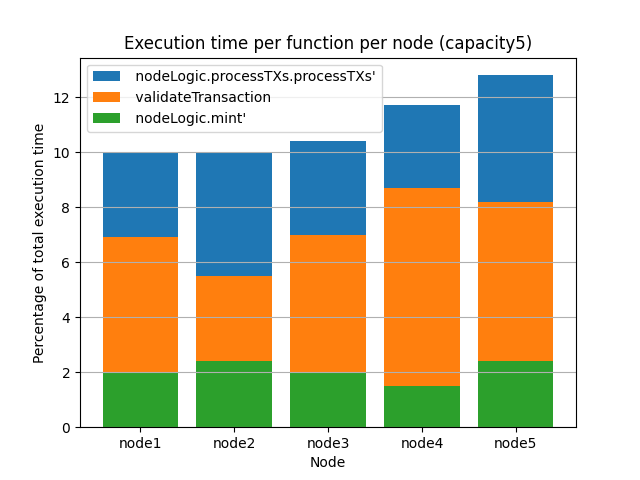
\includegraphics[width=\textwidth]{./capacity5/times_of_function_per_node_capacity5.png}
    \caption{Ποσοστό χρόνου επί του συνολικού χρόνου εκτέλεσης που λαμβάνει η κάθε συνάρτηση \eng{capacity=5}}
    \label{fig:fairness-funcs}
\end{figure}
\FloatBarrier

Στο σχήμα \ref{fig:fairness-funcs} φαίνεται, πράγματι, ότι ο κόμβος με το
μεγαλύτερο \eng{stake} καταναλώνει πολύ περισσότερο χρόνο στην συνάρτηση
\eng{mint'} σε σχέση με τους υπόλοιπους κόμβους, ενδεικτικό του γεγονός ότι
πράγματι αυτός αναλαμβάνει συχνότερα την δημιουργία των νέων \eng{blocks}.
Μάλιστα, επισκοπώντας τα υπόλοιπα των λογαριασμών των κόμβων, παρατηρεί κανείς
ότι όντως τα περισσότερα νομίσματα συσσωρεύονται στον κόμβο με το μεγαλύτερο
\eng{stake}.


\end{document}
